\documentclass[a4paper, 12pt]{article}%тип документа



%отступы
\usepackage[left=1cm,right=1cm,top=1cm,bottom=2cm,bindingoffset=0cm]{geometry}

%%% Работа с русским языком
\usepackage{graphicx}
\usepackage{cmap}                           % поиск в PDF
\usepackage{mathtext} 			 	       % русские буквы в формулах
\usepackage[T2A]{fontenc}               % кодировка
\usepackage[utf8]{inputenc}              % кодировка исходного текста
\usepackage[english,russian]{babel} 
\usepackage{float}
\usepackage{caption}
\usepackage{multirow} 

\usepackage[export]{adjustbox} % локализация и переносы

\usepackage{subfig}% http://ctan.org/pkg/subfig
\usepackage{booktabs}

\usepackage{wrapfig}


%Матеша
\usepackage{amsmath,amsfonts,amssymb,amsthm,mathtools} % AMS
\usepackage{icomma} % "Умная" запятая

%\mathtoolsset{showonlyrefs=true} % Показывать номера только у тех формул, на которые есть \eqref{} в тексте.

%% Шрифты
\usepackage{euscript}	 % Шрифт Евклид
\usepackage{mathrsfs} % Красивый матшрифт

%% Свои команды
\DeclareMathOperator{\sgn}{\mathop{sgn}}

%% Перенос знаков в формулах (по Львовскому)
\newcommand*{\hm}[1]{#1\nobreak\discretionary{}
	{\hbox{$\mathsurround=0pt #1$}}{}}

\date{8 июня 2022 г.}
\author{Гаврилин Илья \\
	Б01-101}
\title{\textbf{Модель Сазерленда,\\исследование теплопроводности воздуха}}

\begin{document}
	\maketitle
	При подсчете эффективного сечения молекулы зачастую рассматривается ее радиус для образования цилиндра в котором больше не может находиться центров молекул, при таком методе оценке применяется формула: $\sigma = \pi d^2$, где $d$ - диаметра молекул.
	Однако, такая модель представляет молекулы в качестве шариков, не рассматривая силы притяжения между ними, тем самым занижая значение эффективного сечения молекулы. Поэтому предлагается рассмотреть иную столкновений молекул, предложенную Сазерлендом\footnote{В некоторой литературе Сёзерленд, англ. Sutherland} в 1893 году. 
	\section{Модель Сазерленда}
	Модель Сазерленда, как уже упоминалось, учитывает силы притяжения между молекулами, при этом на близком расстоянии считая из твердыми шариками.
	\begin{figure}[H]
		\centering
		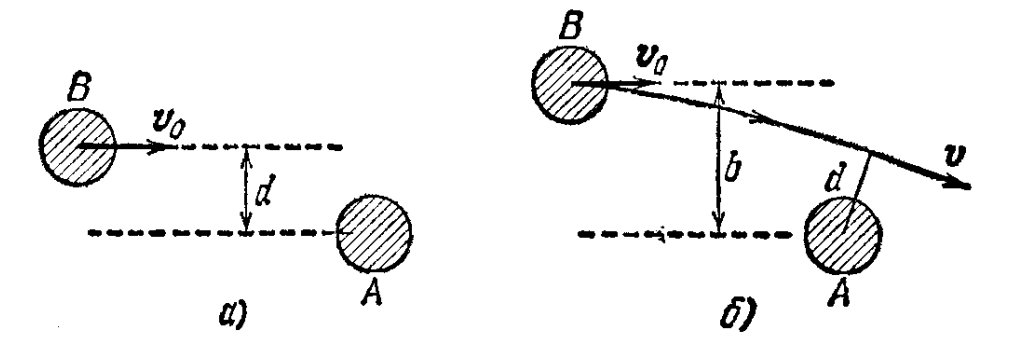
\includegraphics[width=0.8\linewidth]{model}
		\caption{а - модель без учета сил притяжения, б - модель Сазерленда}
		\label{fig:model}
	\end{figure}
	Рассмотрим молекулы А и В, при этом молекула А покоится, а молекула В летит с некоторой скоростью $v_0$ относительно А. Для начала рассмотрим модель, где молекулы представляют из себя твердые шарики диаметра $d$ - случай а. Рассмотрим также ситуацию при наличии сил притяжения тогда за счет данных сил молекулы могут сблизиться на расстояние меньшее или равное их диаметру. $b$ - максимальное расстояние соударения молекул при учете сил притяжения. Отсюда наше эффективное сечение будет равно: $\sigma = \pi b^2, \sigma_0 = \pi d^2$, $\sigma_0$ - эффективное сечение без учета сил притяжения.\\
	Ввиду того, что силы центральные: $v_0 b = v d$, возведя в квадрат: $\sigma v_{0} ^{2} = \sigma_0 v^{2}$ \\
	Из закона сохранения энергии: $\frac{\mu v^2}{2}=\frac{\mu v_0^2}{2} + A$, где $\mu$ - приведенная масса молекул, $A$ - работа центральных сил при перемещении В с "бесконечности" в положение максимального сближения.\\
	Введем кинетическую энергию относительного движения: $\epsilon_{отн} = \frac{\mu v_0^2}{2}$\\
		$$\sigma \epsilon_{отн} = \sigma_0 (\epsilon_{отн} + A)$$
		$$\sigma  = \sigma_0 (1+ \frac{A}{\epsilon_{отн}})$$
	Так как, $\epsilon_{отн} \propto T$, получим: $\sigma  = \sigma_0 (1+ \frac{S}{T})$, где $S$ - постоянная Сазерленда.
	\section{Особенности применения модели Сазерленда}
	Вывод формулы для эффективного сечения, непосредственно потребовал от нас ограничиться столкновением лишь двух частиц, притом что другие частицы отстоят от них на достаточном расстоянии, чтобы силами притяжения от них можно бы было пренебречь. Итого: \textbf{модель Сазерленда справедлива для достаточно разряженного газа, молекулярные силы притяжения убывают с увеличением расстояния между взаимодействующими молекулами достаточно быстро.}
	\section{Учет модели Сазерленда при расчете коэффициента теплопроводности}
	Для потока энергии: $\overline{q} = -k \nabla T$, где k -коэффициент теплопроводности.
	Вспомним, что 
	
	\begin{eqnarray*}
		N^{+} = \frac16 n(x-\lambda)\overline{v} \tau \\
		N^{-} = \frac16 n(x+\lambda) \overline{v} \tau.
	\end{eqnarray*}
	
	Будем считать, что перемещения газа как целого вдоль оси $x$ нет. Тогда $N^{+} = N^{-}$. Пусть $E(x) = c_V T(x)$ - энергия молекулы в точке $x$, а $c_V$ - теплоемкость одной молекулы. Тогда по определению теплового потока:
	
	\begin{equation*}
		q = \frac{ E(x- \lambda)N^{+} - E(x+\lambda) N^{-}}{\tau} = - N^{+} \frac{2\lambda}{\tau} \frac{dE(x)}{dx} = -\frac13 n\overline{v} \lambda c_V \frac{dT}{dx} \Rightarrow k = \frac13 n \overline{v} \lambda c_V
	\end{equation*}
	Напрямую, здесь применить модель Сазерленда стоит в длине свободного пробега:
	$$\lambda = \frac{1}{n \sigma} = (n \sigma_0 (1+ \frac{S}{T}))^{-1}$$
	Итого:
	$$k = k_0 \frac{T_0 + S}{T + S} (\frac{T}{T_0})^{\frac{3}{2}}$$
	где, $k_0$ - теплопроводность газа при температуре $T_0$
	\section{Применение модели Сазерленда при изучении теплопроводности воздуха}
	В течении семестра на лабораторном практикуме была выполнена работа об определении коэффициента теплопроводности воздуха при различных температурах. В ходе работы было получены соответствующие значения теплопроводности:
	\begin{table}[H]
		\centering
		\begin{tabular}{|c|c|c|c|c|c|}
			\hline
			T, K    & 295    & 303    & 313    & 323    & 333    \\ \hline
			$k_{эксп}$ & 0.0253$\pm 0.0023$ & 0.0255$\pm 0.0022$ & 0.0259$\pm 0.0027$ & 0.0281$\pm 0.0029$ & 0.0284$\pm 0.0028$ \\ \hline
		\end{tabular}
	\end{table}
	В данном случае не столь важен ход работы и методы получения данного результата, как важна проверка справедливости модели.\\
	В лабораторной работе было предложено представить зависимость теплоемкости от температуры как: $k(T) \propto T^\alpha$, где в ходе эксперимента выяснили $\alpha = 0.83$
	Построим график с указанием полученных значений теплопроводностей и прямыми соответствующими моделям предоставленным: в лабораторной работе - степенной, модели Сазерленда(S = 120 K).
	\begin{figure}[H]
		\centering
		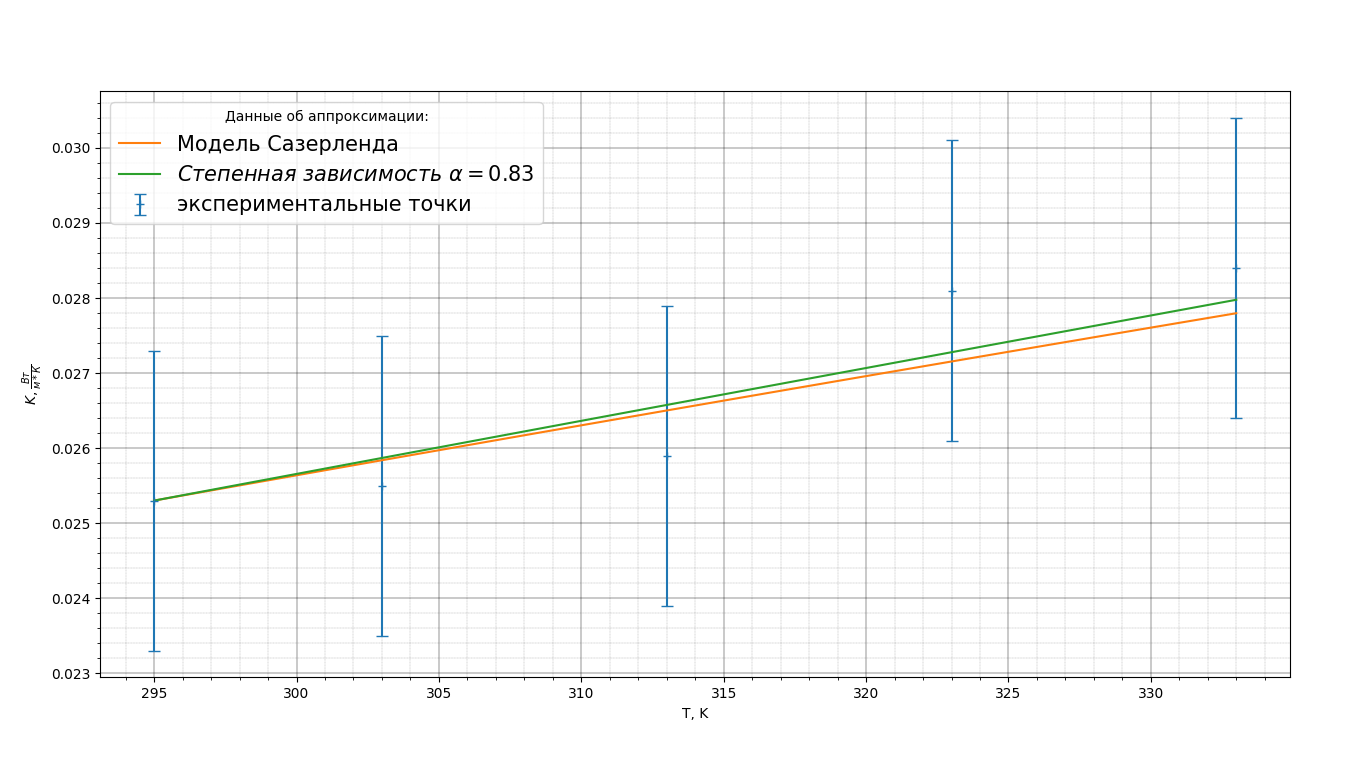
\includegraphics[width=0.95\linewidth]{Figure_1}
		\caption{Зависимость коэффициента теплопроводности от температуры}
		\label{fig:figure1}
	\end{figure}
	Можем заметить, что обе модели хорошо описывают теплопроводность газов при условиях, близких к нормальным. Модель сазерленда показывает несколько более заниженные значения коэффициента теплопроводности, однако, заметим справедливость применения данной модели к описанию теплопроводности воздуха. Большую разницу можно заметить на более высоких температурах, где вклад притяжения будет более заметен.
\end{document}
